% !TeX root = ../thuthesis-example.tex

\chapter{混合车队队列稳定性分析}
\label{sec:3}

\section{人工驾驶车辆扰动传递函数推导}

人工驾驶车辆的跟驰行为由速度优化模型(OVM)描述,其具体表达式为
\begin{align}
  \dot{v}_n(t) &= \kappa \left\{ \mathrm{V} \left[ h_n(t) \right] - v_n(t) \right\} \notag \\
  \mathrm{V} \left[ h_n(t) \right] &= v_0 \left\{ 1 - \exp \left[ - \frac{\alpha}{v_0}\left(h_n(t)-s_0\right) \right] \right\}
  \label{eq:chap03-1}
\end{align}
其中,各符号含义在表\ref{tab:chap01-5}中给出,其相关参数取值如表\ref{tab:chap02-1}所示。

当车队整体处于均衡状态时,车队中所有车辆加速度都保持为0,所有车辆都保持均衡速度$v_e$行驶。对于人工驾驶车辆,说明速度优化函数与车队均衡速度相同,即
\begin{equation}
  \mathrm{V}[h_e] = v_e
  \label{eq:chap03-2}
\end{equation}
其中$h_e$为均衡状态下自动驾驶车辆与前车的距离,称作均衡速度。将速度优化函数带入式(\ref{eq:chap03-2}),得到式(\ref{eq:chap03-3})。
\begin{equation}
  v_0 \left\{ 1 - \exp \left[ -\frac{\alpha}{v_0} (h_e - s_0) \right] \right\} = v_e
  \label{eq:chap03-3}
\end{equation}
整理得到均衡距离与均衡速度之间的关系,如式(\ref{eq:chap03-4})所示。
\begin{equation}
  h_e = s_0 - \frac{v_0}{\alpha}\ln\left( 1 - \frac{v_e}{v_0} \right)
  \label{eq:chap03-4}
\end{equation}
\begin{figure}
  \centering
  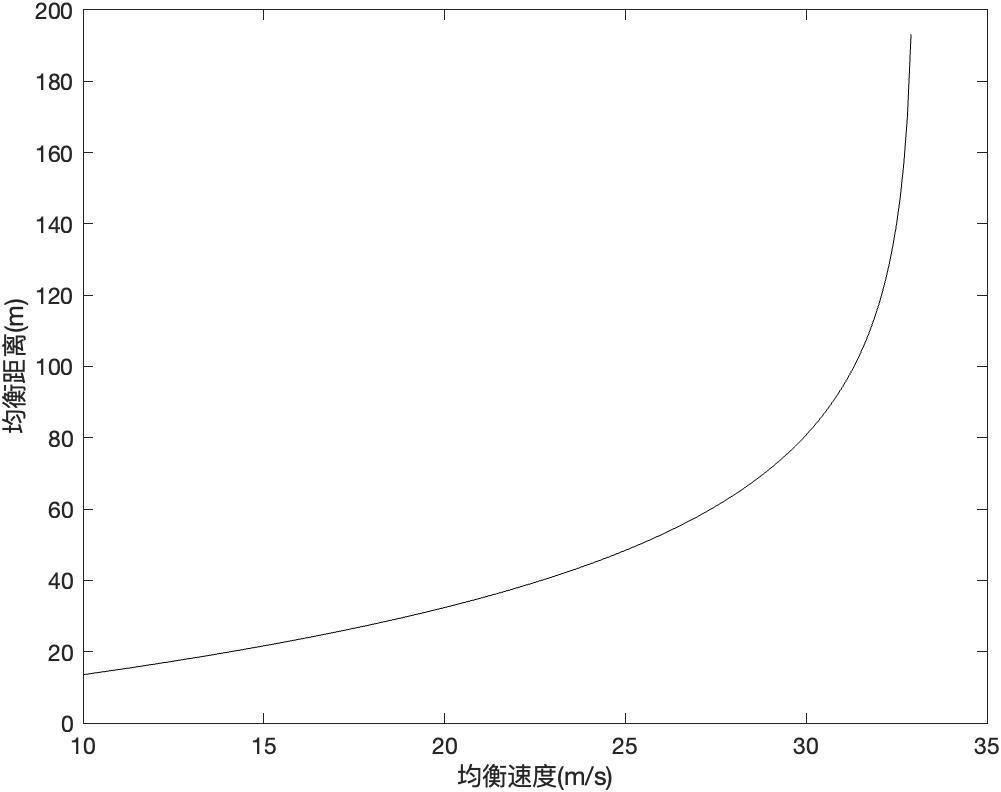
\includegraphics[width=0.5\linewidth]{chap03-1.jpg}
  \caption{OVM均衡距离与均衡速度关系曲线}
  \label{fig:chap03-1}
\end{figure}

图\ref{fig:chap03-1}描述了均衡距离与均衡速度的关系,从中可以看出OVM的均衡距离与均衡速度呈正相关,均衡速度越大,两车之间的均衡距离也越大,这说明当速度较大时,驾驶员倾向于
增大与前车的距离以减小追尾的风险。同时也可以看出随着均衡速度的增加,均衡距离的增长速度也越来越快。

下面对OVM的人工驾驶车辆对扰动的传递情况进行分析。假设车队受到扰动,第$n-1$辆车和第$n$辆车的扰动为
\begin{equation}
  \begin{cases}
    \increment{v_{n-1}(t)} = v_{n-1}(t) - v_e \\
    \increment{v_n(t)} = v_n(t) - v_e
  \end{cases}
  \label{eq:chap03-5}
\end{equation}
对等式两边同时求导,可以发现扰动函数的导函数与速度函数的导函数是相同的,即
\begin{equation}
  \begin{cases}
    \increment{\dot{v}_{n-1}(t)} = \dot{v}_{n-1}(t) \\
    \increment{\dot{v}_n(t)} = \dot{v}_n(t)
  \end{cases}
  \label{eq:chap03-6}
\end{equation}
将式(\ref{eq:chap03-1})中加速度函数中的速度优化函数在$h_n(t)=h_e$处一阶泰勒展开,得到式(\ref{eq:chap03-7})
\begin{equation}
  \increment{\dot{v}}_n(t) = \dot{v}_n(t) = \kappa \left\{ \mathrm{V'}(h_e)[h_n(t)-h_e] - v_n(t) \right\}
  \label{eq:chap03-7}
\end{equation}
等式两边同时求导,得到
\begin{equation}
  \begin{aligned}
    \increment{\ddot{v}}_n(t) &= \kappa \left[ \mathrm{V'}(h_e)\dot{h}_n(t) - \dot{v}_n(t) \right] \\
                              &= \kappa \left\{ \mathrm{V'}(h_e)\left[v_{n-1}(t) - v_n(t)\right] - \dot{v}_n(t) \right\} \\
                              &= \kappa \left\{ \mathrm{V'}(h_e)\left[\increment{v_{n-1}(t)} - \increment{v_n(t)} \right] - \increment{\dot{v}_n(t)} \right\}
  \end{aligned}       
  \label{eq:chap03-8}
\end{equation}
等式两边同时做拉普拉斯变换(因为是在均衡状态下添加的扰动,所以满足零初始条件),得到
\begin{equation}
  s^2\increment{V}_n(s) = \kappa \left\{ \mathrm{V'}(h_e)\left[\increment{V_{n-1}(s)} - \increment{V_n(s)} \right] - s\increment{V_n(s)} \right\}
  \label{eq:chap03-9}
\end{equation}
整理得到速度扰动在OVM下的传递函数$G_{H}(s)$如式(\ref{eq:chap03-10})所示。
\begin{equation}
  G_{H}(s) = \frac{\increment{V_{n}(s)}}{\increment{V_{n-1}(s)}} = \frac{\kappa V'(h_e)}{s^2 + \kappa s + \kappa V'(h_e)}
  \label{eq:chap03-10}
\end{equation}

\section{自动驾驶车辆扰动传递函数推导}

自动驾驶车辆的跟驰行为由基于PID控制的车头时距控制算法控制,该算法的表达式为
\begin{equation}
  \dot{v}_n(t) = k_1 \left[ h_n(t) - l - t_hv_n(t) \right] + k_2 \left[ v_{n-1}(t) - v_n(t) \right]
  \label{eq:chap03-11}
\end{equation}
其中,各符号含义在表\ref{tab:chap02-2}中给出

下面对自动驾驶车辆对扰动的传递情况进行分析。与人工驾驶车辆分析过程相同,假设车队受到扰动,第$n-1$辆车和第$n$辆车的扰动为
\begin{equation}
  \begin{cases}
    \increment{v_{n-1}(t)} = v_{n-1}(t) - v_e \\
    \increment{v_n(t)} = v_n(t) - v_e
  \end{cases}
  \label{eq:chap03-12}
\end{equation}
扰动函数的导函数与速度函数的导函数是相同的,即
\begin{equation}
  \begin{cases}
    \increment{\dot{v}_{n-1}(t)} = \dot{v}_{n-1}(t) \\
    \increment{\dot{v}_n(t)} = \dot{v}_n(t)
  \end{cases}
  \label{eq:chap03-13}
\end{equation}
对式(\ref{eq:chap03-11})两边同时求导,得到
\begin{equation}
  \begin{aligned}
    \increment{\ddot{v}}_n(t) &= \ddot{v}_n(t) = k_1 [\dot{h}_n(t) - t_h\dot{v}_n(t)]
                              + k_2 [\dot{v}_{n-1}(t) - \dot{v}_n(t)] \\
    &= k_1 [\dot{h}_n(t) - t_h \increment{\dot{v}_n(t)}]
       + k_2 [\increment{\dot{v}_{n-1}(t)} - \increment{\dot{v}_n(t)}] \\
    &= k_1 [\increment{v}_{n-1}(t) - \increment{v}_n(t) - t_h \increment{\dot{v}_n(t)}]
       + k_2 [\increment{\dot{v}_{n-1}(t)} - \increment{\dot{v}_n(t)}] \\
  \end{aligned}
  \label{eq:chap03-14}
\end{equation}
等式两边同时做拉普拉斯变换,得到
\begin{equation}
  \begin{aligned}
    s^2\increment{V}_n(s) = &k_1[ \increment{V_{n-1}(s)} - \increment{V_{n}(s)} - t_hs\increment{V_{n}(s)}] \\
                            &+ k_2 [ s\increment{V_{n-1}(s)} - s\increment{V_n(s)} ]
  \end{aligned}
  \label{eq:chap03-15}
\end{equation}
整理得到速度扰动在自动驾驶车辆的传递函数$G_{A}(s)$如式(\ref{eq:chap03-16})所示。
\begin{equation}
  G_{H}(s) = \frac{\increment{V_{n}(s)}}{\increment{V_{n-1}(s)}} = 
  \frac{k_2s + k_1}{s^2 + (k_1t_h + k_2) s + k_1}
  \label{eq:chap03-16}
\end{equation}

\section{混合车队跟驰行为稳定性分析}
\label{sec:3.3}

首先给出队列稳定性的定义。 \\

\begin{definition}[队列稳定(String Stable)]
  对于一个跟驰车队,如果头车受到扰动后,扰动沿着车队逐渐衰减,认为该车队是队列稳定的。
  \label{def:chap03-def1}
\end{definition}

根据\ref{sec:1.2.2}中对车队稳定性分析研究现状的调研,得到只包含一种传递函数的车队的队列稳定性充分条件为
\begin{equation}
  | G(j\omega) | < 1
  \label{eq:chap03-17}
\end{equation}
其中$G(j\omega)$是该车队含有的唯一一种传递函数。这个充分条件其实是由式(\ref{eq:chap03-18})简化而来的。
\begin{equation}
  | G(j\omega) |^n < 1
  \label{eq:chap03-18}
\end{equation}
其中$n$是车队中跟驰车辆的数量。

对于含有两种及两种以上传递函数的车队,比如本工作中人工驾驶车辆和自动驾驶车辆有不同的传递函数,车队队列稳定的充分条件是
\begin{equation}
  \left\Vert \prod_{i=1}^{m}{G_i(j\omega)^{p_i}} \right\Vert_{\infty} < 1
  \label{eq:chap03-19}
\end{equation}
其中,车队中传递函数共有$m$种,第$i$种传递函数对应的车辆在车队跟驰车辆中的比例为$p_i$。

对于本工作的情景,队列稳定的条件可以简化为
\begin{equation}
  \left\Vert G(j\omega) \right\Vert_{\infty} = \left\Vert G_H(j\omega)^{1-p} \cdot G_A(j\omega)^p \right\Vert_{\infty} < 1
  \label{eq:chap03-20}
\end{equation}

需要说明的是,只有在车队中每一辆跟驰车辆都严格按照其跟驰模型行驶的情况下,式(\ref{eq:chap03-20})才能保证车辆绝对队列稳定,该队列稳定性的判据的价值更多
体现在理论层面,因为在真实场景下,跟驰车辆并不会严格按照某一个跟驰模型行驶,即使是自动驾驶车辆,也会因为计算误差、传感器精确度、计算延迟等众多实际因素产生
与其控制算法的误差,更何况真实场景下,交通环境中存在大量的随机性。

对于本工作,如\ref{sec:simulation-platform}中提到的,在搭建仿真平台时,为了追求更加接近真实场景的仿真,加入了加速度限制、人类驾驶员反应延迟、一阶惯性环节等
使仿真跟驰行为不同于其跟驰模型的因素,使得仿真环境也是不同于每一辆跟驰车辆都严格按照其跟驰模型行驶的理想情况的。

但这并不意味着以上的推导是没有意义的,一方面,混合车队的队列稳定性充分条件的推导具有理论价值;另一方面,对于仿真场景或真实场景,式(\ref{eq:chap03-20})中
$\left\Vert G(j\omega) \right\Vert_{\infty}$的值仍能反应车队的队列稳定情况,即在真实场景中,满足式(\ref{eq:chap03-20})可以说明该车队在理论上队列稳定,
但真实场景下仍然有出现扰动被不断放大的可能,即便如此,我们仍可以用$\left\Vert G(j\omega) \right\Vert_{\infty}$的值作为一个指标对车队的队列稳定性进行评估。


\section{混合车队跟驰行为稳定性仿真验证}
\label{sec:3.3}

在本小节中,将通过仿真的方式对\ref{sec:3.3}中理论推导的结果进行验证。需要说明的是,本小节的仿真分为两部分,一部分是理想情况仿真,是对理论推导结果的验证,在仿真过程中没有加入\ref{sec:simulation-platform}
中提到的加速度限制、人类驾驶员反应延迟、一阶惯性环节等使仿真跟驰行为不同于其跟驰模型的因素;另一部分是模拟真实场景仿真,在仿真过程中加入了使仿真跟驰行为不同于其跟驰模型的因素,是为了说明式(\ref{eq:chap03-20})
得到的指标确实可以反应模拟真实场景下车队的稳定性。

\subsection{车队稳定情况仿真}

理论上,队列稳定的车队在受到扰动后,扰动会逐渐减小,最终趋于0。下面选取一个场景对车队稳定的情况进行仿真。\\

经验证,在自动驾驶车辆占比为0.5,初始均衡速度为$25m/s$的条件下,$\left\Vert G(j\omega) \right\Vert_{\infty} = \left\Vert G_H(j\omega)^{0.5} \cdot G_A(j\omega)^{0.5} \right\Vert_{\infty} < 1$,
即理论上车队是稳定的。

\begin{figure}
  \centering
  \subcaptionbox{理想情况仿真 \label{fig:chap03-2-stable-ideal}}
    {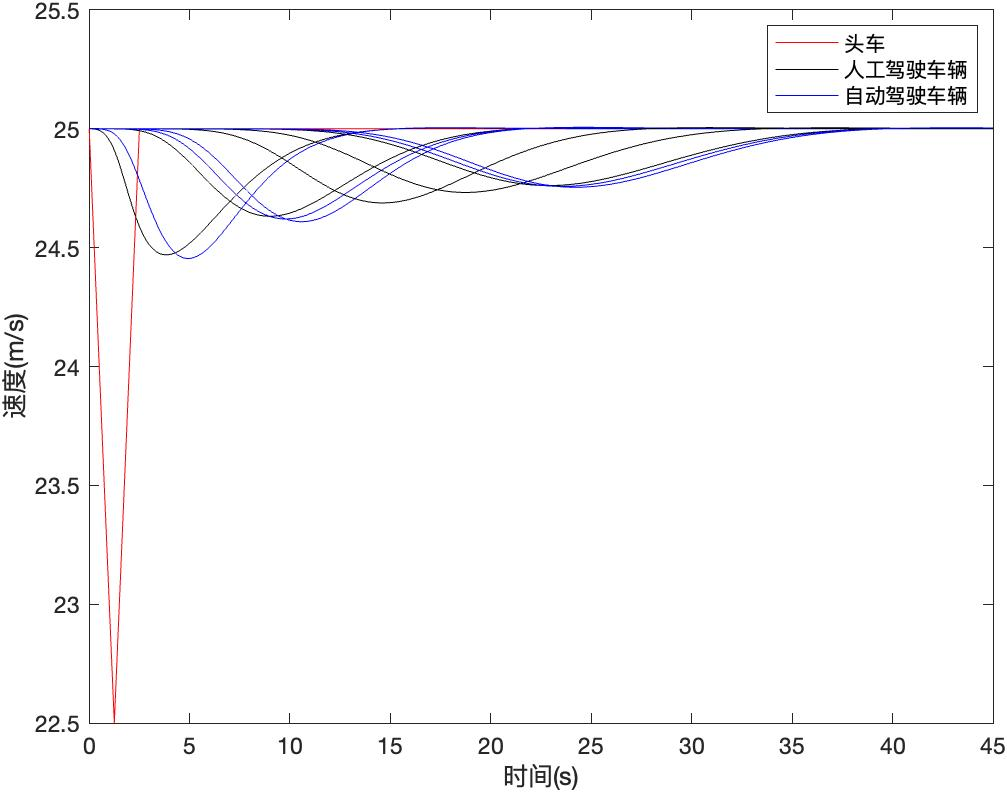
\includegraphics[width=0.47\linewidth]{chap03-2-ideal-0.5-25.jpg}}
  \subcaptionbox{模拟真实场景仿真 \label{fig:chap03-2-stable-real}}
    {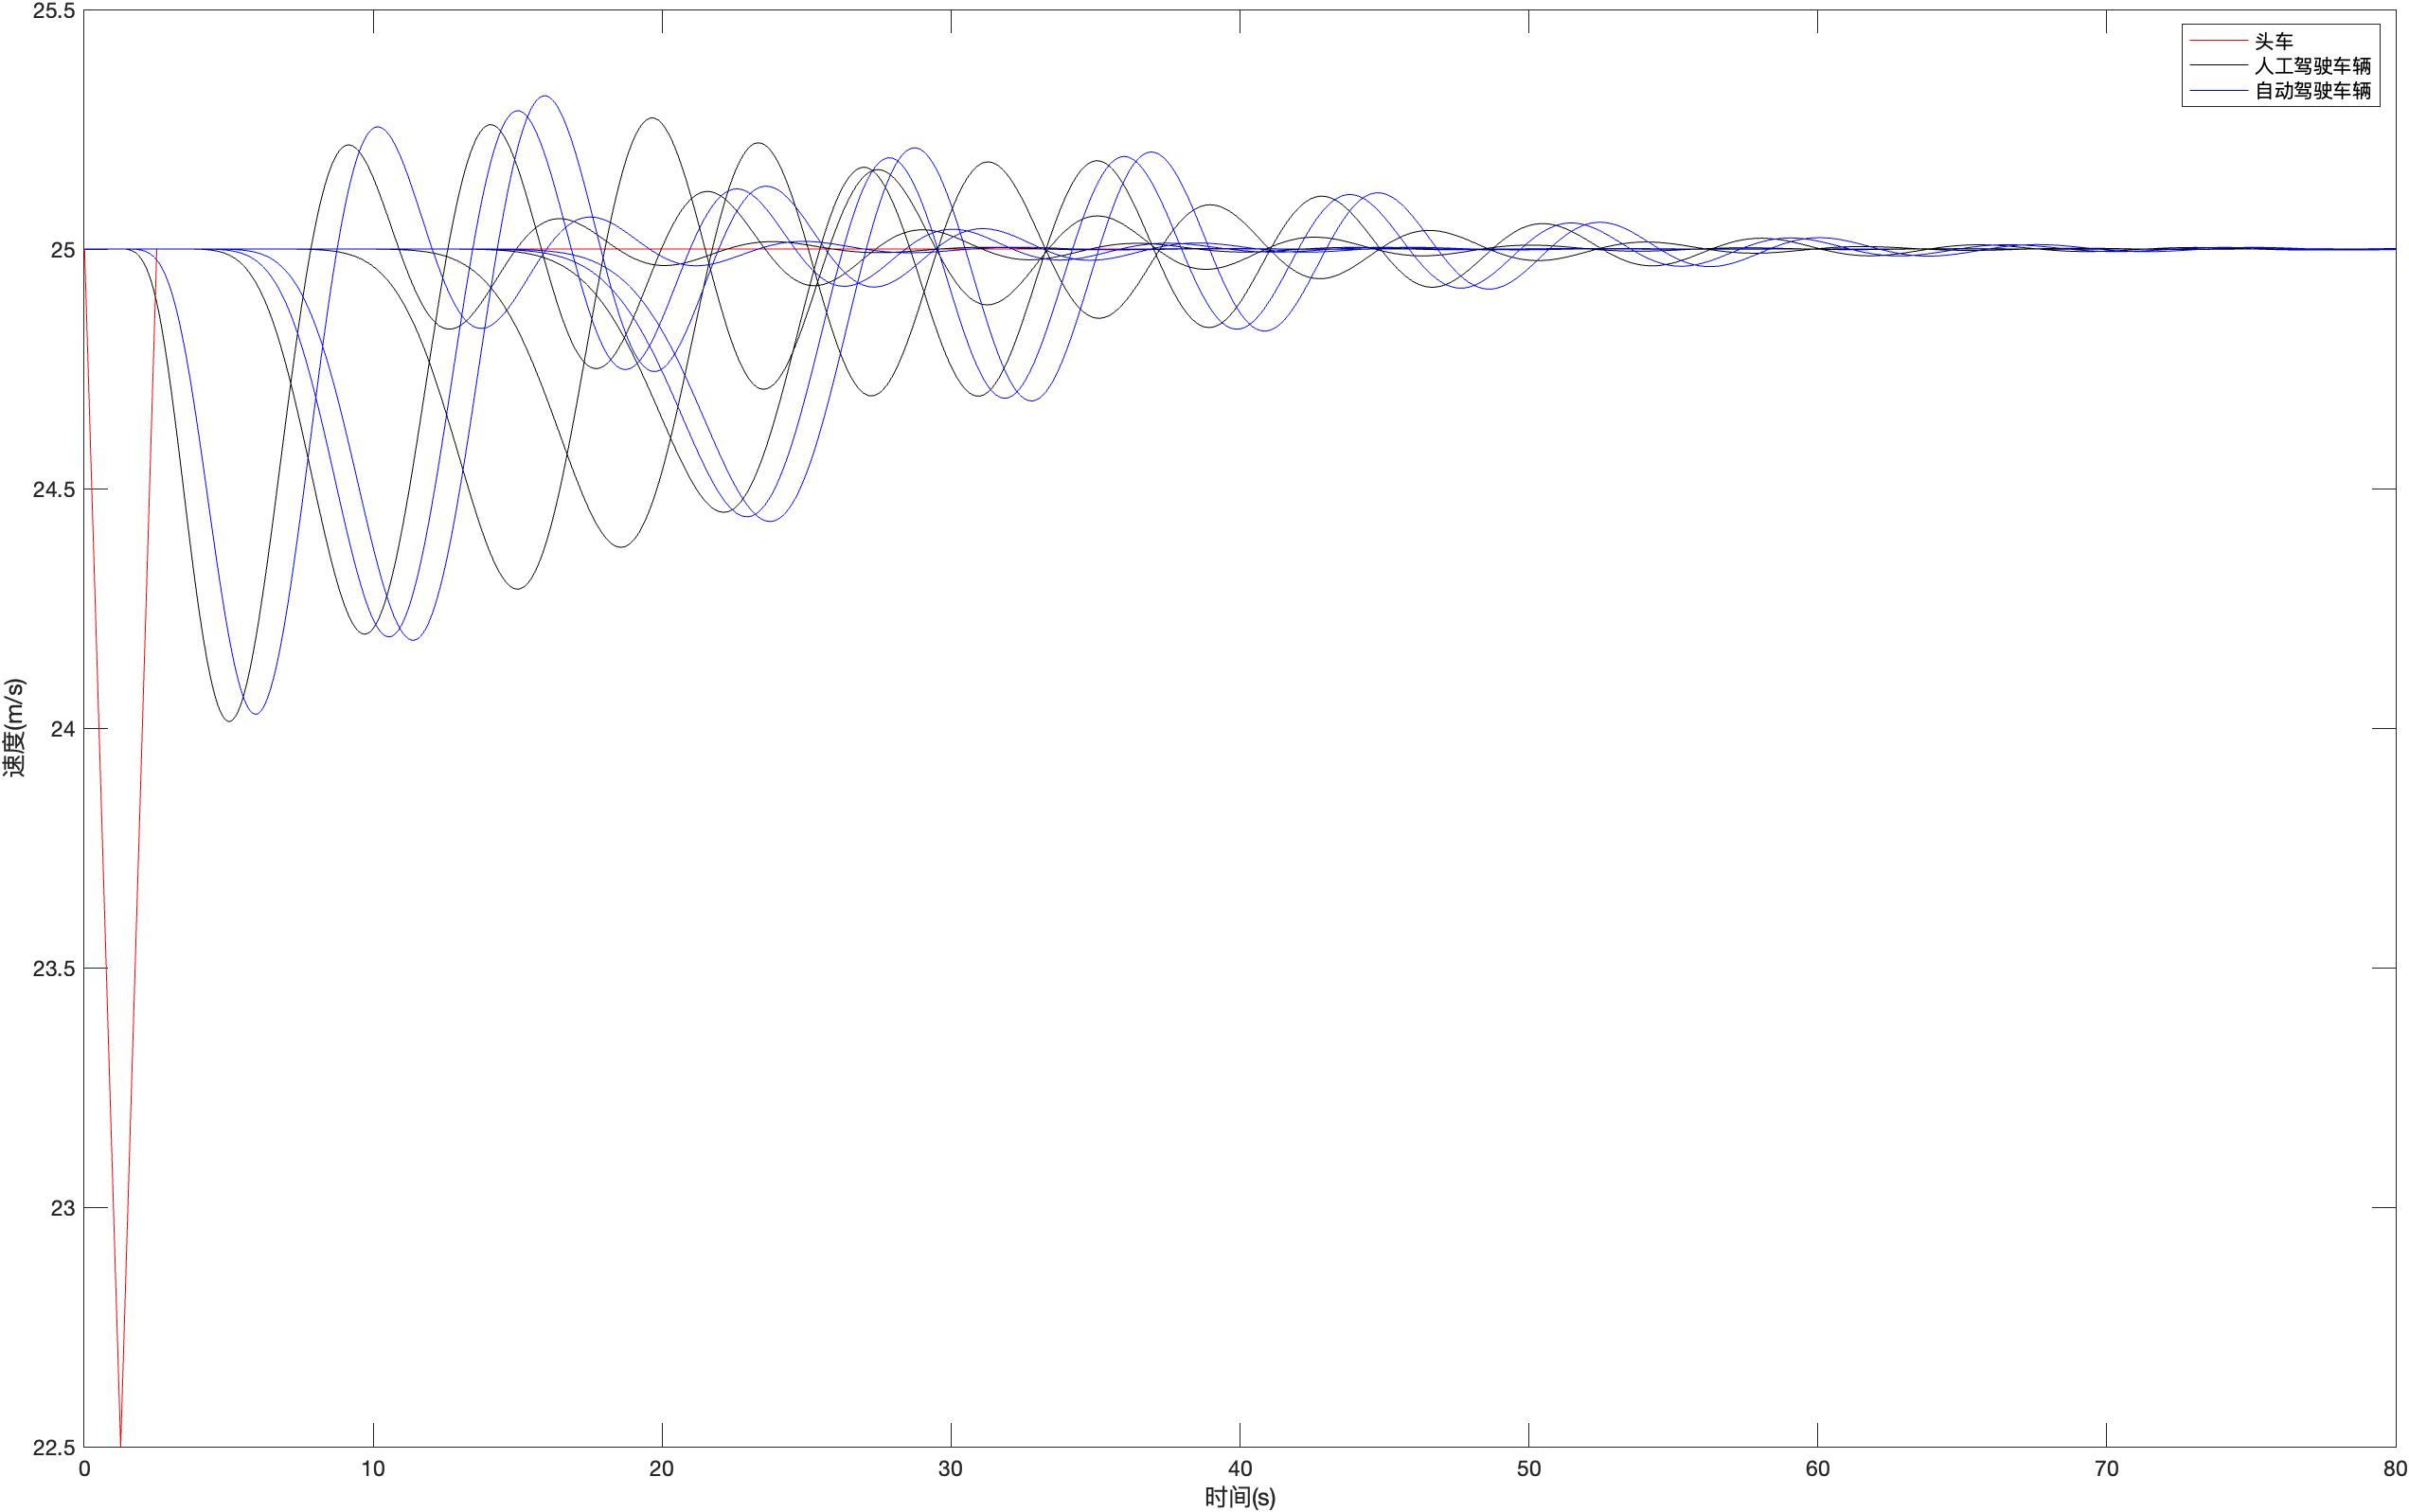
\includegraphics[width=0.52\linewidth]{chap03-2-real-0.5-25.jpg}}
    \caption*{在理想情况仿真中,车队中每辆跟驰车辆严格按照跟驰模型行驶;在模拟真实场景仿真中,加入了加速度限制、人类驾驶员反应延迟、一阶惯性环节等因素}
    \caption{车队稳定情况仿真}
  \label{fig:chap03-2}
\end{figure}

可以观察到无论是在理想情况仿真中还是在模拟真实场景仿真中,衰减都沿着车队逐渐衰减,这说明二者对应的车队都是稳定的。

\subsection{车队不稳定情况仿真}
\label{sec:3.4.2}

经验证,在自动驾驶车辆占比为0.3,初始均衡速度为$10m/s$的条件下,$\left\Vert G(j\omega) \right\Vert_{\infty} = \left\Vert G_H(j\omega)^{0.7} \cdot G_A(j\omega)^{0.3} \right\Vert_{\infty} > 1$,
即理论上车队是不稳定的。

\begin{figure}
  \centering
  \subcaptionbox{理想情况仿真 \label{fig:chap03-3-unstable-ideal}}
    {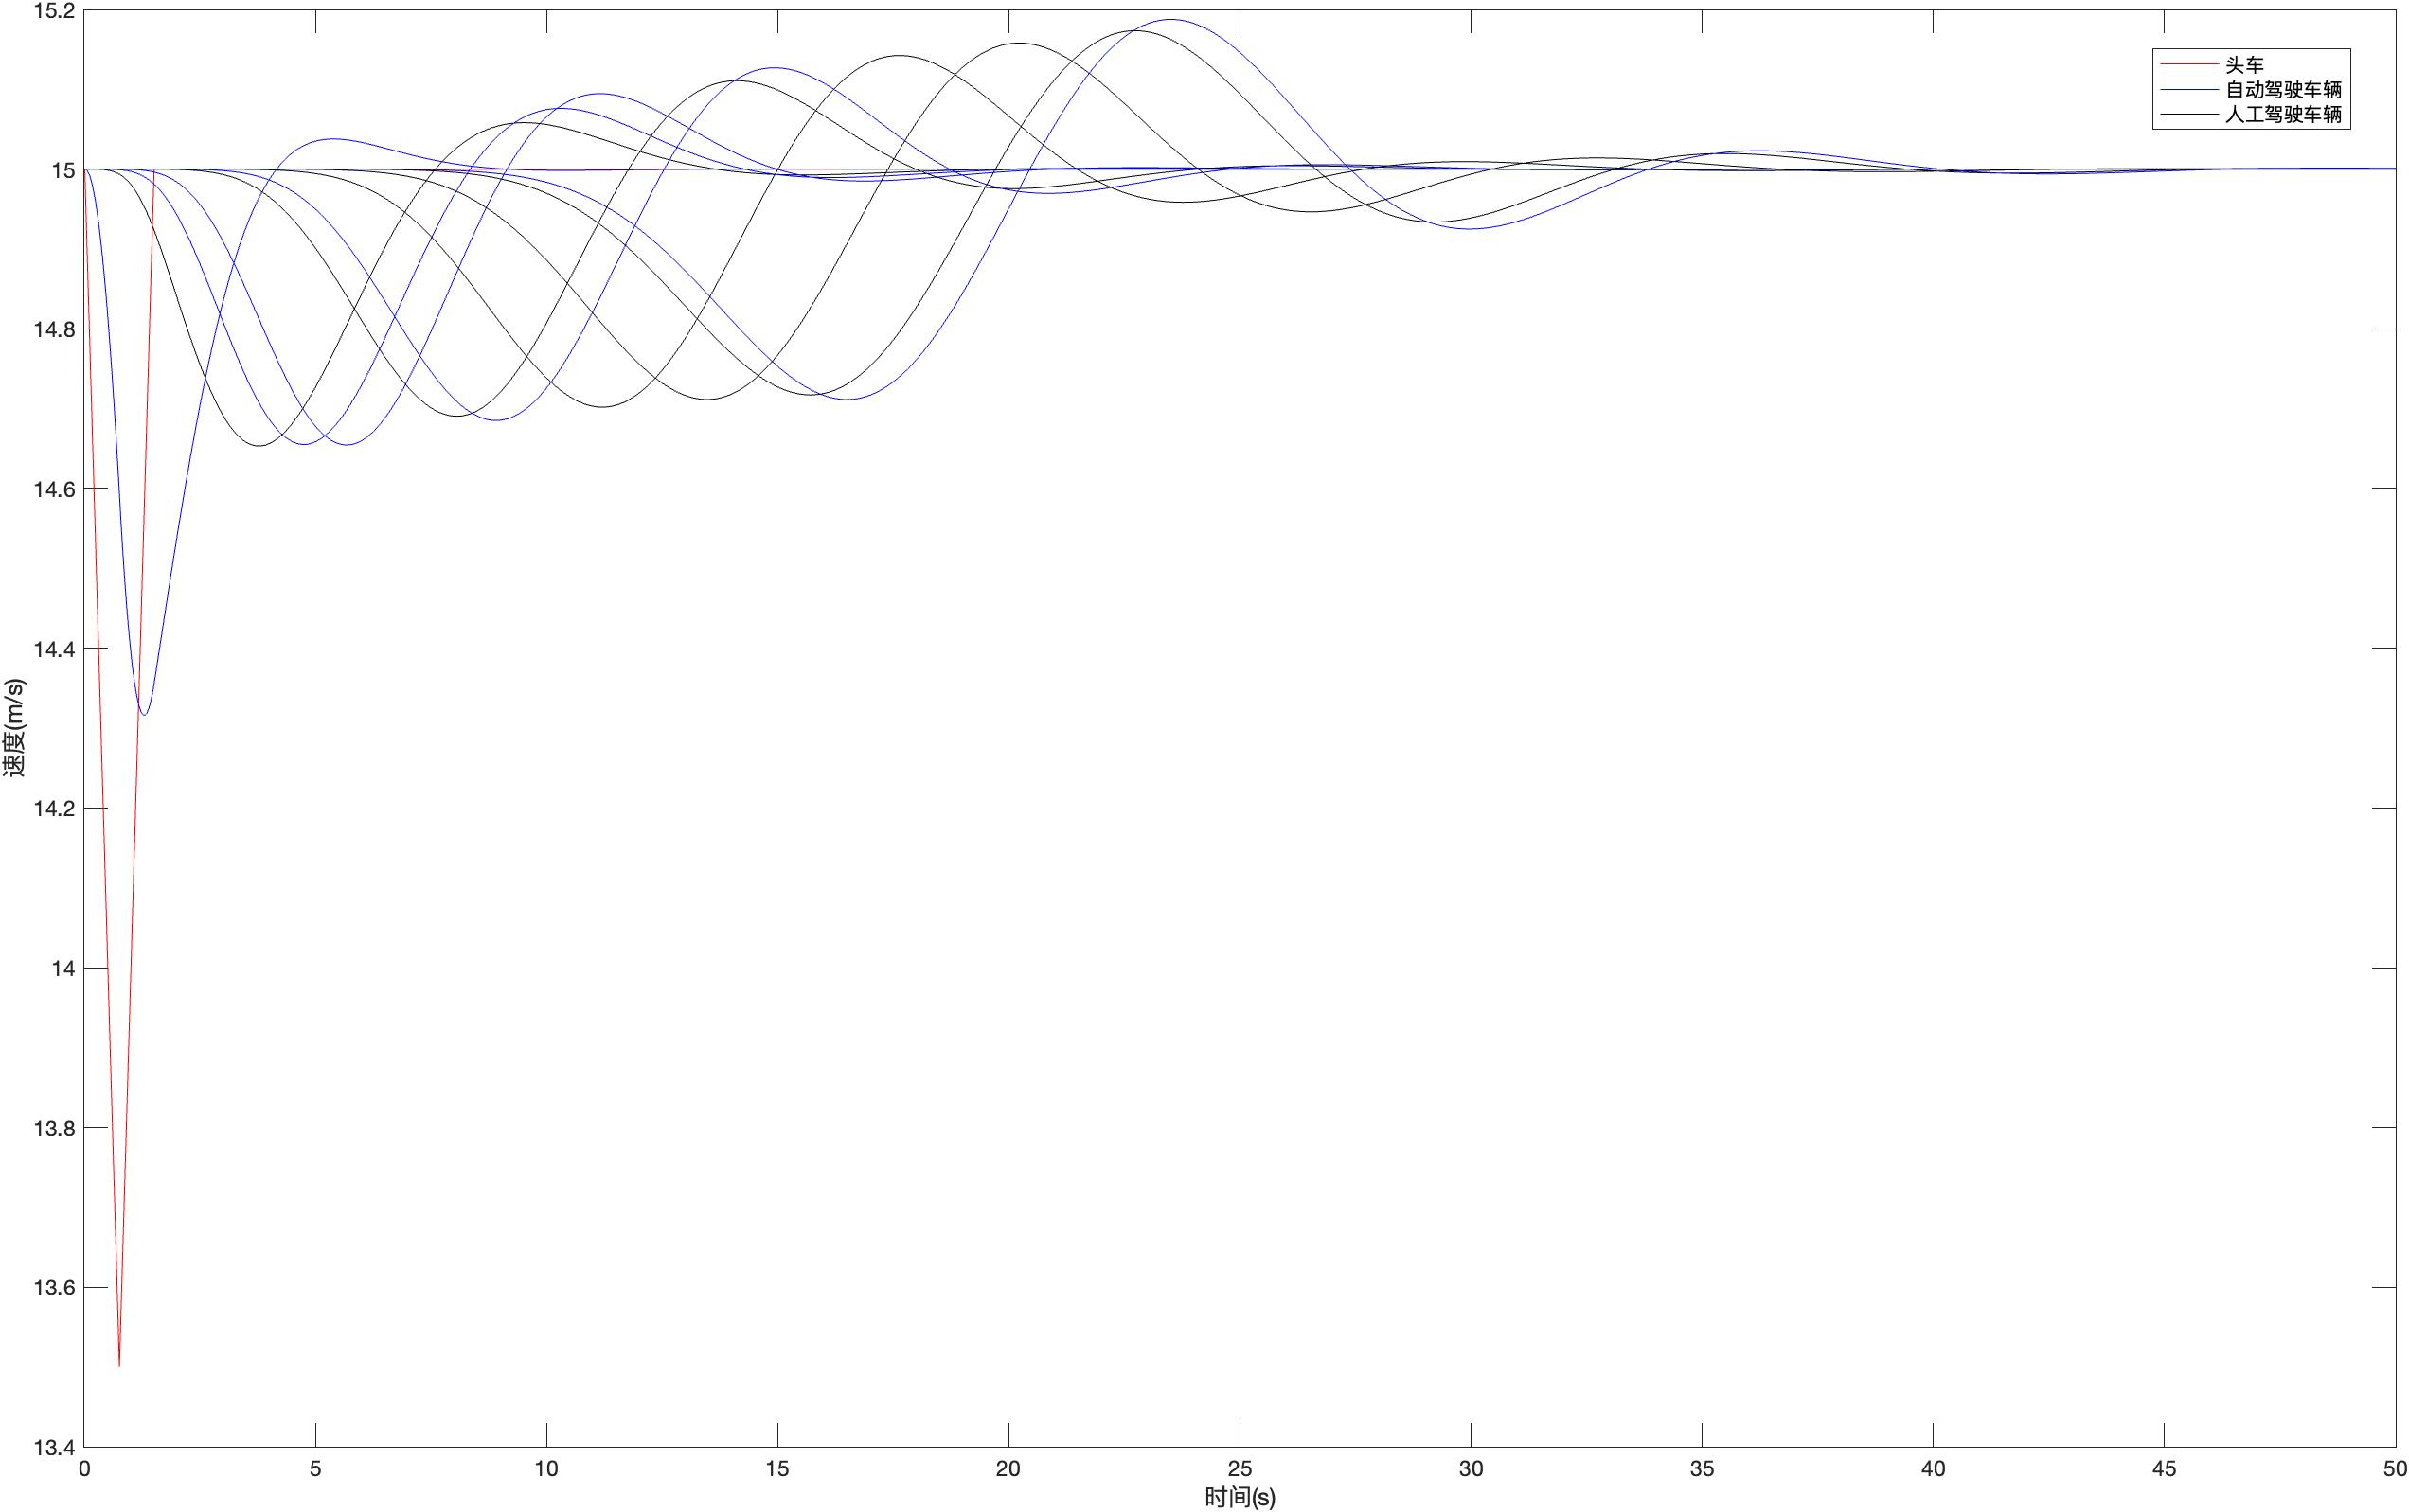
\includegraphics[width=0.5\linewidth]{chap03-2-ideal-0.5-15.jpg}}
  \subcaptionbox{模拟真实场景仿真 \label{fig:chap03-3-unstable-real}}
    {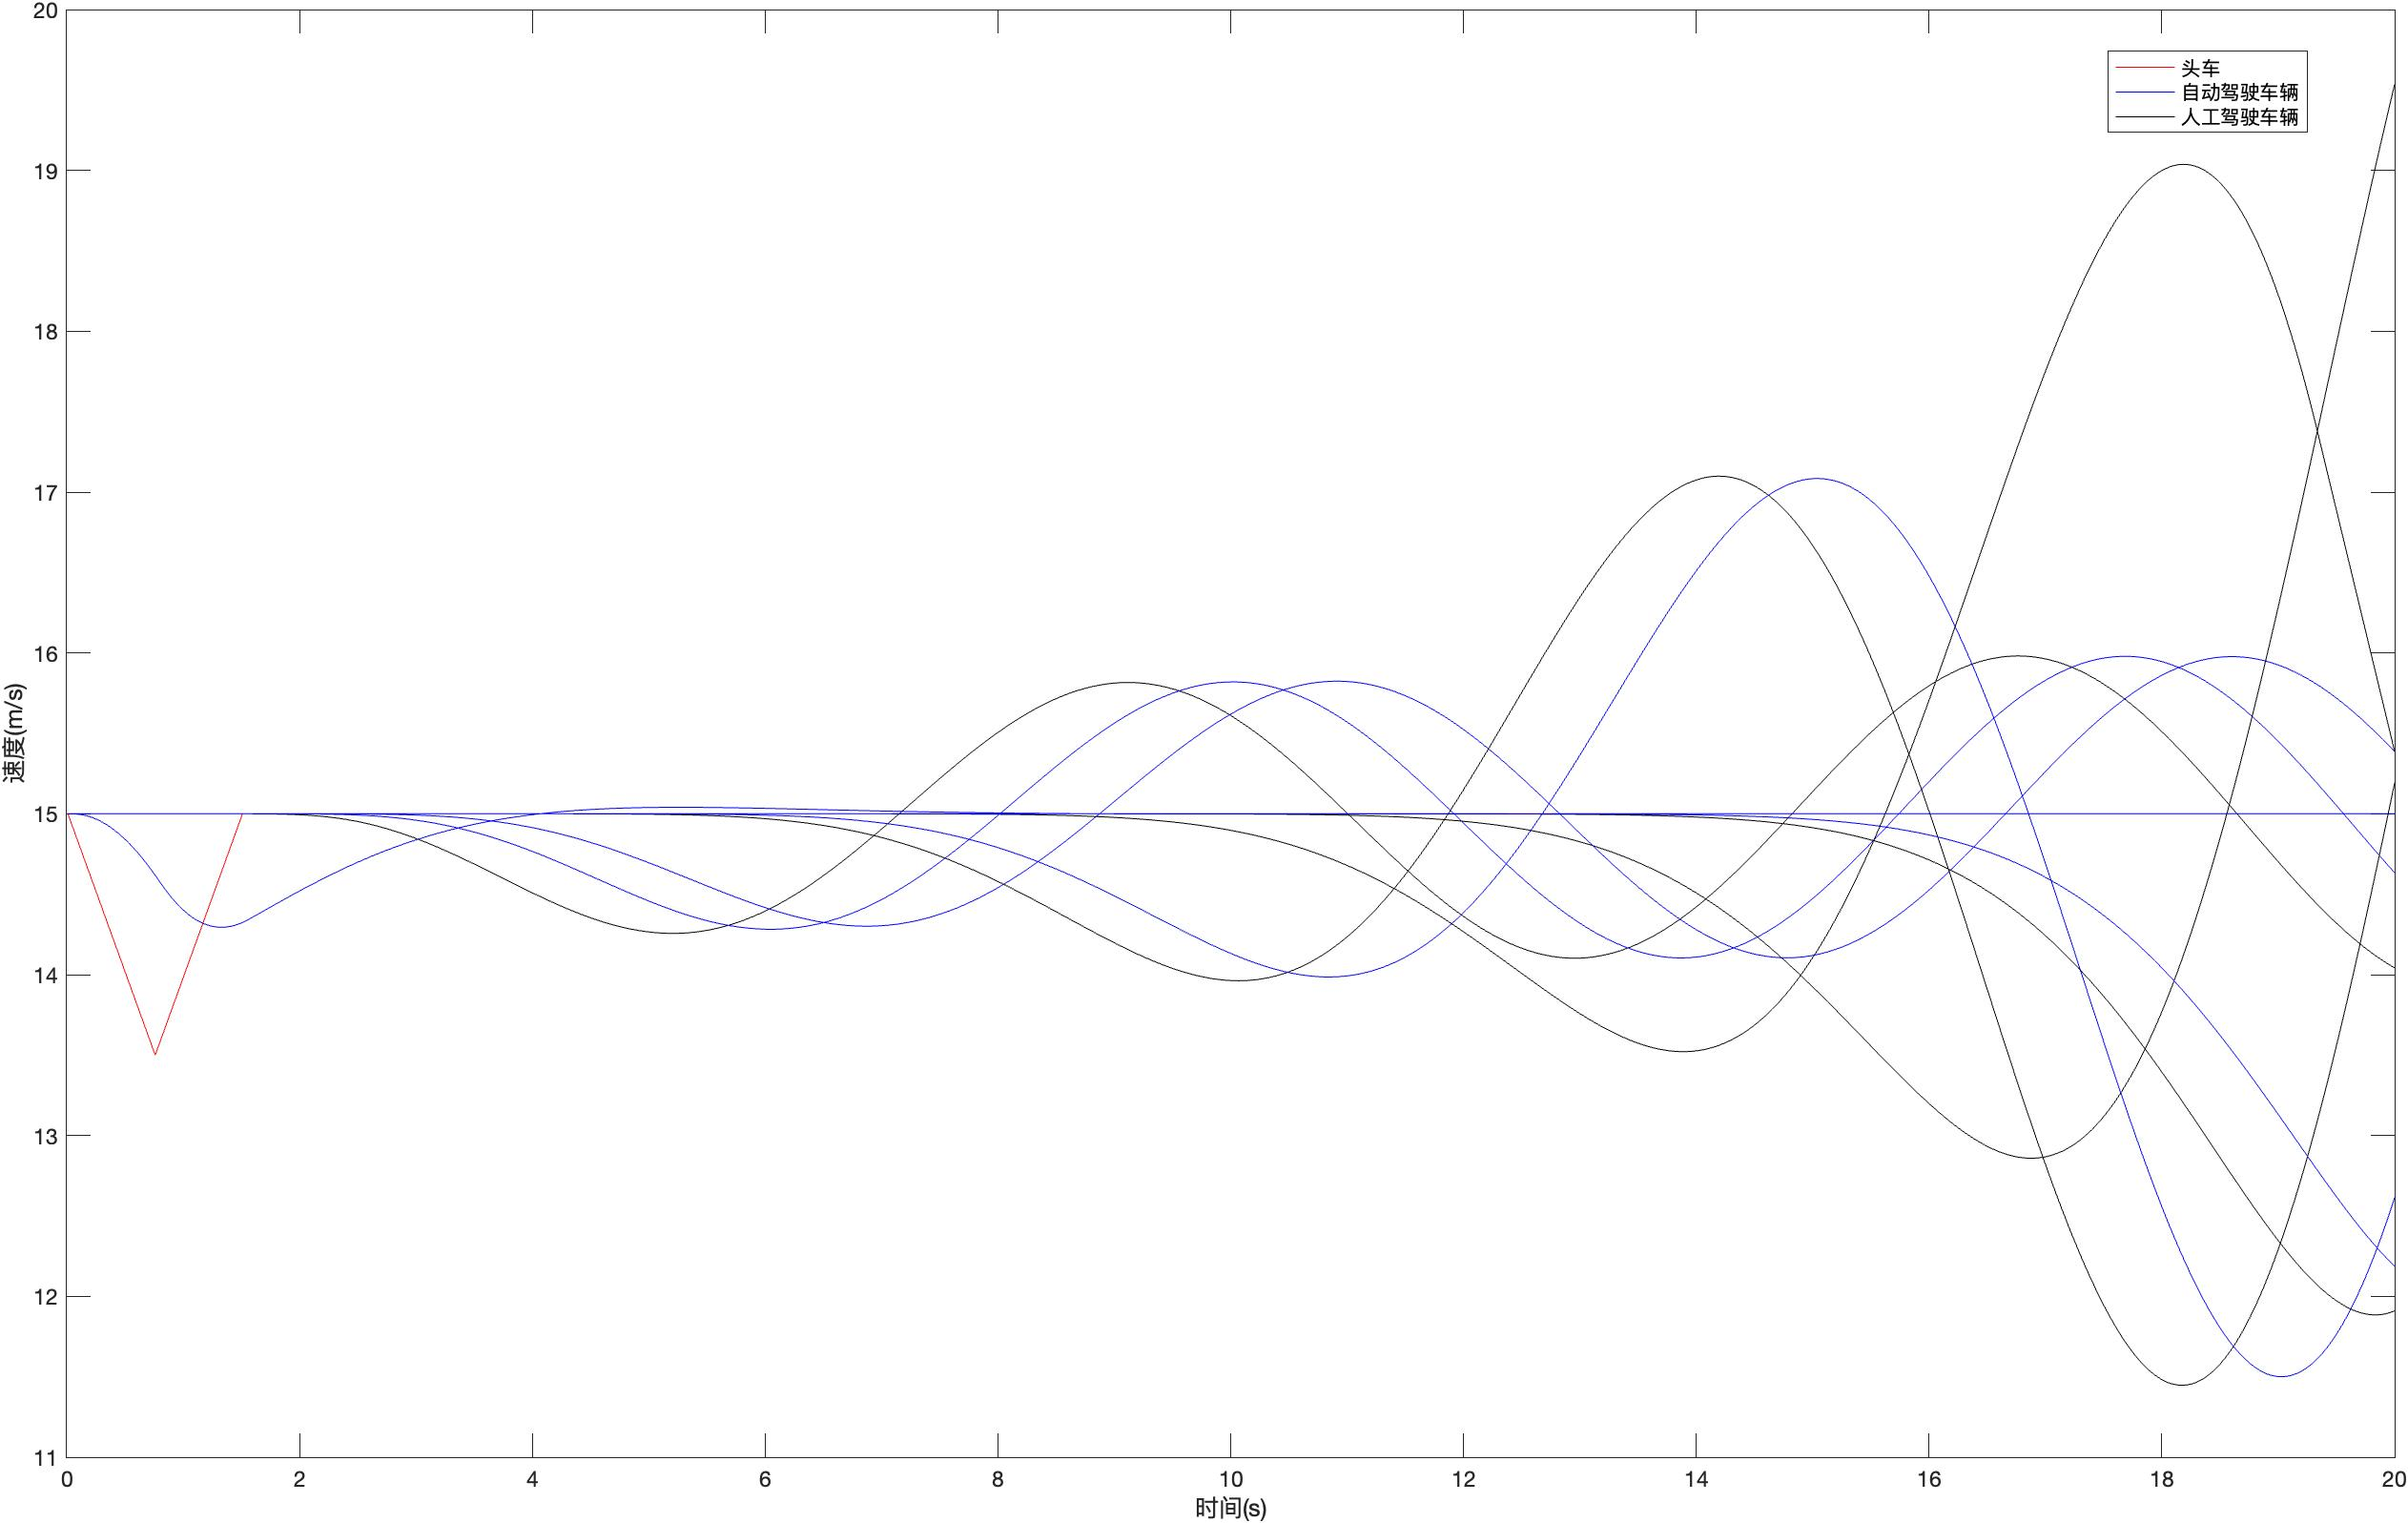
\includegraphics[width=0.5\linewidth]{chap03-3-real-0.5-15.jpg}}
    \caption*{在理想情况仿真中,车队中每辆跟驰车辆严格按照跟驰模型行驶;在模拟真实场景仿真中,加入了加速度限制、人类驾驶员反应延迟、一阶惯性环节等因素}
    \caption{车队不稳定情况仿真}
  \label{fig:chap03-3}
\end{figure}

可以观察到在理想情况仿真中,虽然随着时间的推移,车队中每辆车的扰动都趋于0,但从空间角度来看,衰减沿着车队被放大,通过队列稳定性的定义,可以确定这个车队是队列不稳定的。而
对于模拟真实场景仿真中,衰车队呈现出更不稳定的状态,扰动最终发散,在这样的车队中极容易发生事故。

但在图\ref{fig:chap03-2}和图\ref{fig:chap03-3}所示的场景中,理想情况仿真和模拟真实场景仿真都具有一致的稳定性,虽然这并不意味着理想情况和模拟真实场景情况有相同的稳定性,但可以说明
式(\ref{eq:chap03-20})得到的车队传递函数无穷范数即使在考虑了真实场景因素的情况下,也能反应车队整体的队列稳定性。

\section{本章小结}
在本章中,首先对人工驾驶车辆和自动驾驶车辆对扰动对传递情况进行了分析,得到了二者关于扰动大小的传递函数,进而利用队列稳定性这一概念推导得到了理论上车队达到队列稳定的充分条件。但这一条件也存在一定的局限性,
即只有当车队中所有车辆都严格按照其跟驰模型行驶时,才能使用这个判据,而本工作的核心是建立车队稳定性与碰撞风险之间的联系,碰撞风险是基于仿真得到的,如果仿真场景不够真实,则建立的联系就不具备实际价值。所以
在本章的最后对理想情况和模拟真实场景都进行了仿真分析,发现$\left\Vert G(j\omega) \right\Vert_{\infty}$的值能够反应真实场景下车队的稳定程度,也说明了本章进行的稳定性分析工作是有意义的。

图\ref{fig:chap03-4}描述了本章的结构。

\begin{figure}
  \centering
  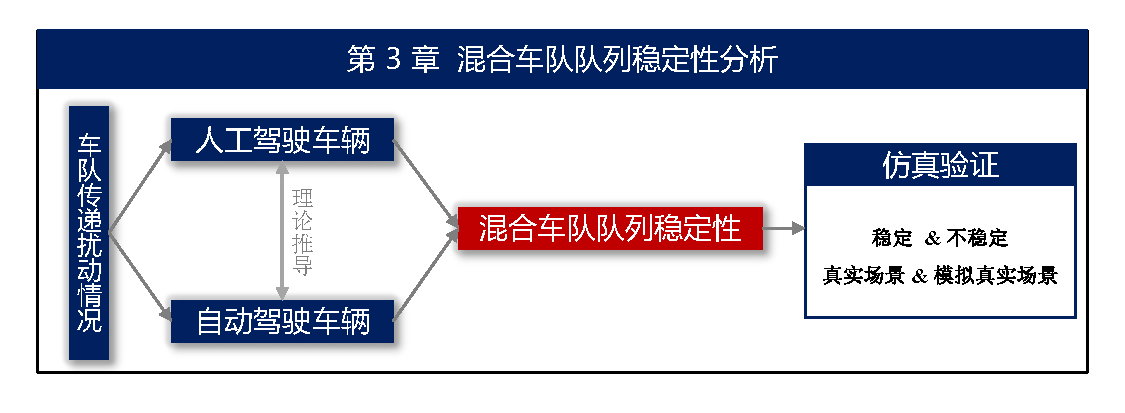
\includegraphics[width=1\linewidth]{chap03-structure.pdf}
  \caption{第3章结构}
  \label{fig:chap03-4}
\end{figure}